\begin{center}
Лабораторная работа №1.
\\
Тема: Работа с системами контроля версий.
\\
Цель: Изучить порядок клонирования репозитория на гитхабе и на компьютере.
 
\end{center}
Задание:
\begin{enumerate}
\item Зарегистрироваться на https://github.com/

\item Склонировать репозиторий шаблонов tex https://github.com/egorpugin/tex
 
\item Подготовить шаблон отчёта для лабораторных работ в LaTeX.

\item Загрузить шаблон в репозиторий tex.

\item Создать новый репозиторий для лабораторных работ на гитхабе.

\item Оформить отчёт и загрузить его в репозиторий для ЛР.
\end{enumerate}
Ход выполнения:
\\
Порядок клонирования репозитория на гитхабе.
\\
\begin{enumerate}
\item Нажать кнопку Fork (Клонировать)
\end{enumerate}

\begin{figure}[h]
\centering
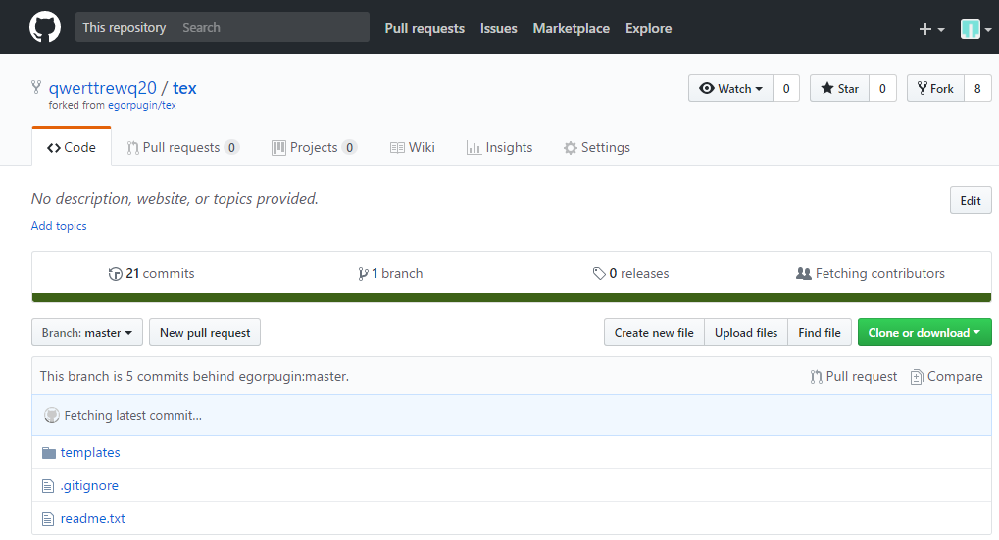
\includegraphics[scale=0.5]{qwe}
\caption{Клонирования репозитория на гитхабе}
\label{fig:qwe}
\end{figure}
 
Порядок клонирования репозитория на компьютере.

\begin{figure}[h]
\centering
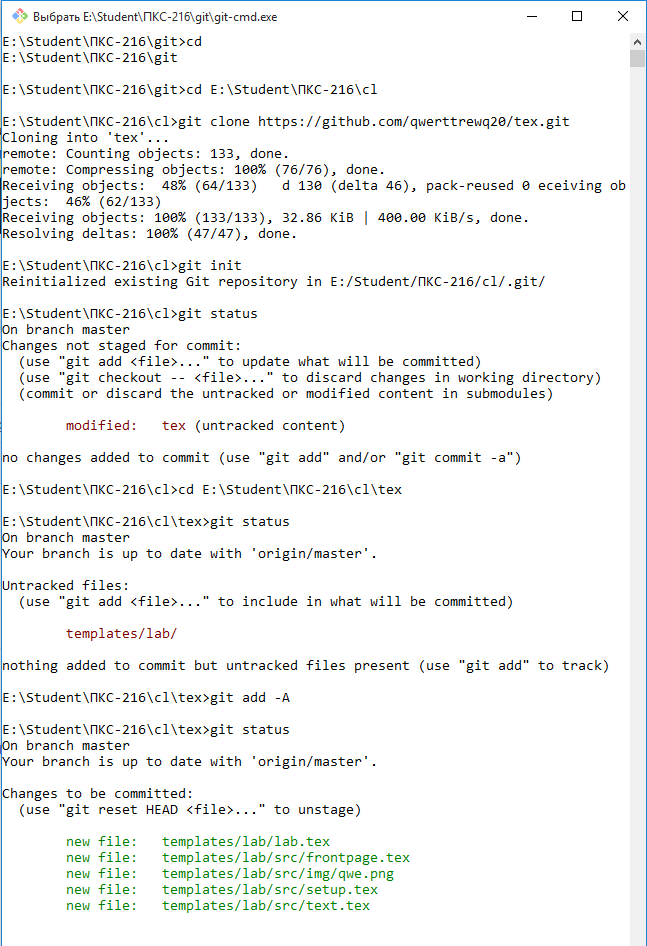
\includegraphics[scale=1]{sk1}
\caption{Клонирования репозитория на компьютер, внесения новых файлов}
\label{fig:sk1}
\end{figure}

\begin{figure}[h]
\centering
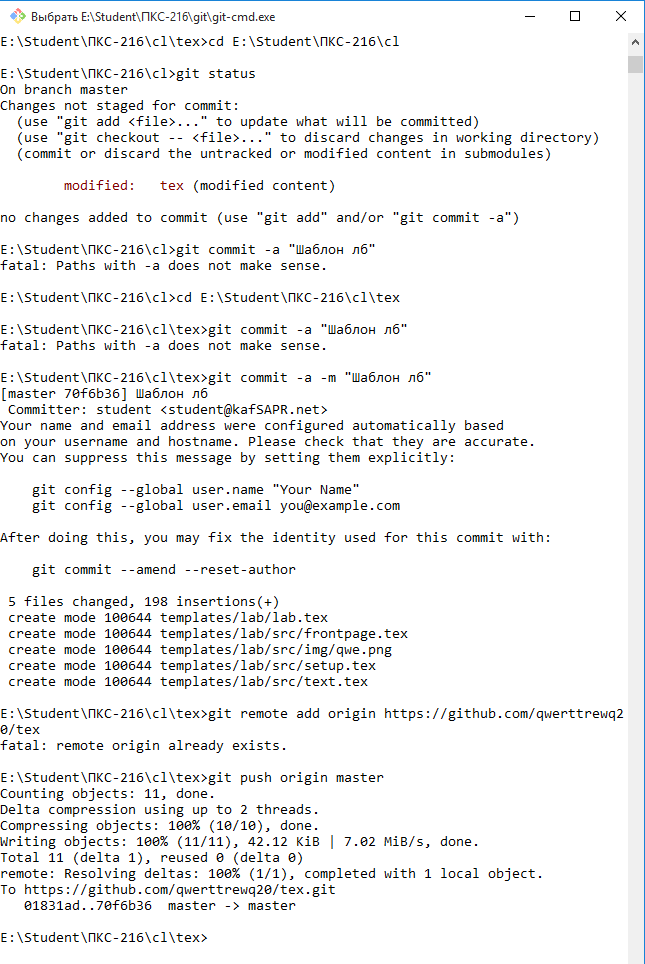
\includegraphics[scale=0.9]{sk2}
\caption{Фиксация изменений и загрузка изменений на гитхаб}
\label{fig:sk2}
Вывод: Изучил порядок клонирования репозитория на гитхабе и на компьютере.
\end{figure}




